\part{Start of the art} \label{part:state_art}

\chapter{What is the Internet of Things?}

The Internet of Things or IoT, also called Internet of Everything, Web of Things, can be viewed as the interconnection of things, often referred as objects, motes or smart objects. The Global Standards Initiative on Internet of Things (IoT-GSI) defined \textit{Internet of Things} as "\textit{a global infrastructure for the information society, enabling advanced services by interconnecting (physical and virtual) things based on existing and evolving interoperable information and communication technologies}"\cite{ituitu}. They also give an explanation about what they consider a \textit{"thing"} to be. A thing is "\textit{an object of the physical world (physical things) or the information world (virtual things), that is capable of being identified and integrated into communication networks}"\cite{ituitu}. Fig.\ref{fig:iot} shows examples of things.\\

\todo[inline]{Give other examples as industry automation or smart cities, or healthcare. (see architecting iot article)}
With the IoT, we dispose of networks constituted by devices which have the ability to communicate between them to exchange data. Also those devices can interact with their environment with means of sensors or actuators. An illustration of such network would be the \textit{Smart Home}. With Smart Home, automation comes into our house. The idea is to have, for example, your door talking to the lights to tell them to light on or to light off depending on if you enter or leave the room. You could have that your alarm would tell the coffee machine to prepare some coffee when ringing in the morning or that your thermostat would regulate the heat of the house. Also, you could remotely manage your house by activating or deactivating the heat and so on. While discussing the present of the IoT in homes, one field that could largely benefit from the IoT is the field of \textit{e-health}, thanks to the medical monitoring of elderly, ill, and disabled patients, while they would still be in their house and keep their autonomy in their daily life. Smart objects could either be implanted in or around the patient, and information is retrieved from their situation to have regular checkups on their condition(s). The information is then sent and analyzed by specialized staff, ready to intervene if needed. The advantage here is having the ability to remotely monitor patients' situation. (source : architecting the iot).\\

\begin{figure}
  \label{fig:iot}
  \centering
  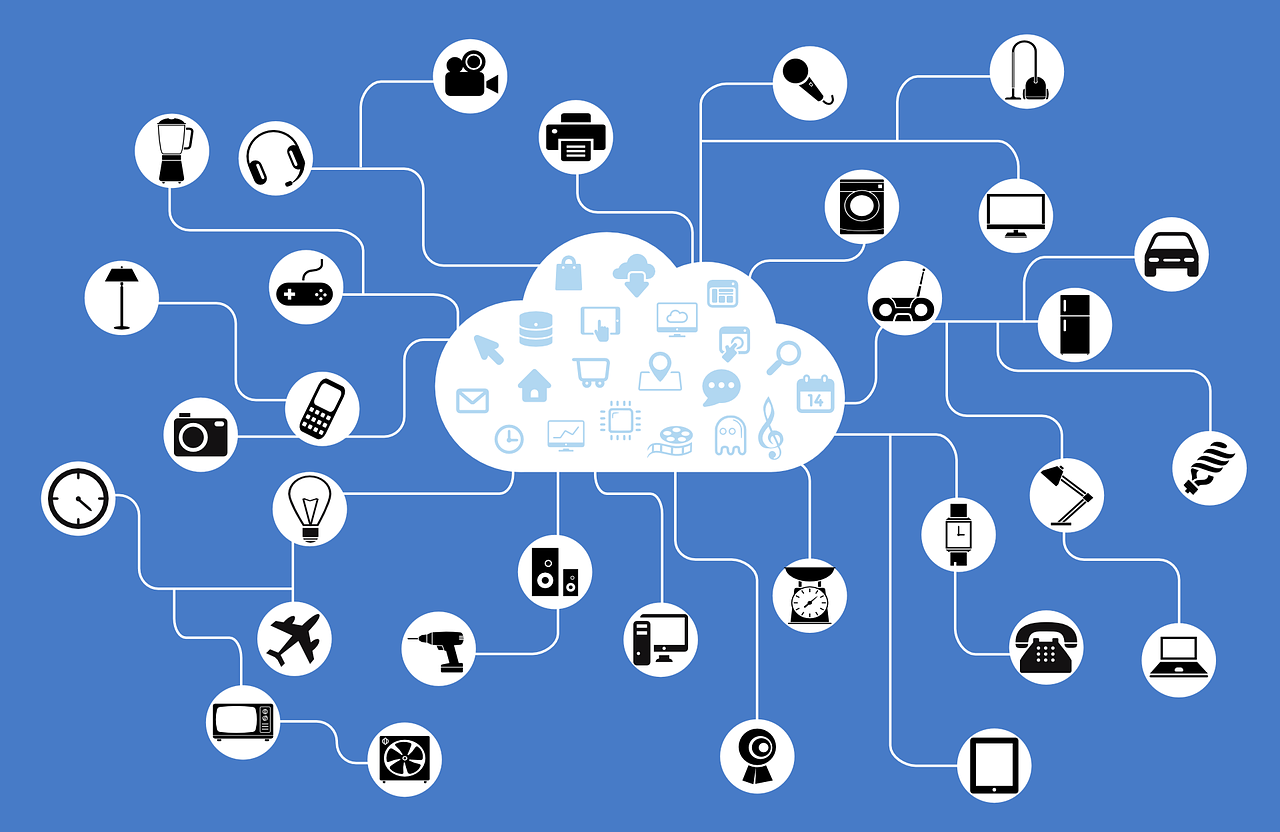
\includegraphics[width=\textwidth]{res/iot.png}
  \caption{Internet of Things (Source: \url{pixabay.com})}
\end{figure}

But IoT is not limited only to home. It is already deployed on organizations. For example, the start-up Epicenter injects microchips into their employees (after agreement)\cite{website:lat_04_17}. The microchip enable an employee to open a door or to operate a printer by just a wave of the hand. Also it permits to track them inside the building and permits a colleague to know your whereabouts. \\

The Internet of Things can also be used in many more situations. Power grids can now be better controlled and managed with smart objects, the temperature in buildings and houses can now be monitored and smart objects control radiators and air conditioners to modify ambient temperature, and thus make a more efficient consumption of energy. Shipping containers could also be equipped with devices to better help monitor and modify the climate inside, thus making sure food, clothing, and various materials are better taken care of. Environments hard to analyse like glacier or mountains becomes easier to monitor as we only need to place sensors nodes that will periodically send us the data retrieved from the environment such as temperature. \\

\todo[inline]{Speak about \textit{Industrial Revolution} and \textit{Industry 4.0}}

Those examples show how much we could benefit from IoT. It could improve our efficiency in term of energy. But also could make our life easier by automating certain aspects of the life. In the following subsections, we will go deeper into some technical aspects of the Internet of Things. \\

\todo[inline]{Challenges of iot : preface of book (page xx) + slide 17 du premier cours de mobile.}


\section{Smart Objects}

Smart objects are the main components of an IoT Network. We will explain what makes them special and the purpose of their use.\\

Smart objects, also called IoT Devices, smart devices or connected devices, are physical objects, that are embedded with an electronical component, that allows them to communicate with other objects. Those objects are composed of a software, are equipped with a microprocessor, a sensor or an actuator that allows them to interact with the physical environment and modify/control it, and network connectivity to allow exchange and collection of data. Thanks to network connectivity, devices can sense and exchange sense data of the physical world with each other. They are also often equipped with a small battery, that provides a power source to the device. The connectivity is assured by wireless in most cases. Fig.\ref{fig:smart_objects} shows examples of smart objects.\\

\begin{figure}
    \centering
    \begin{subfigure}[b]{0.3\textwidth}
        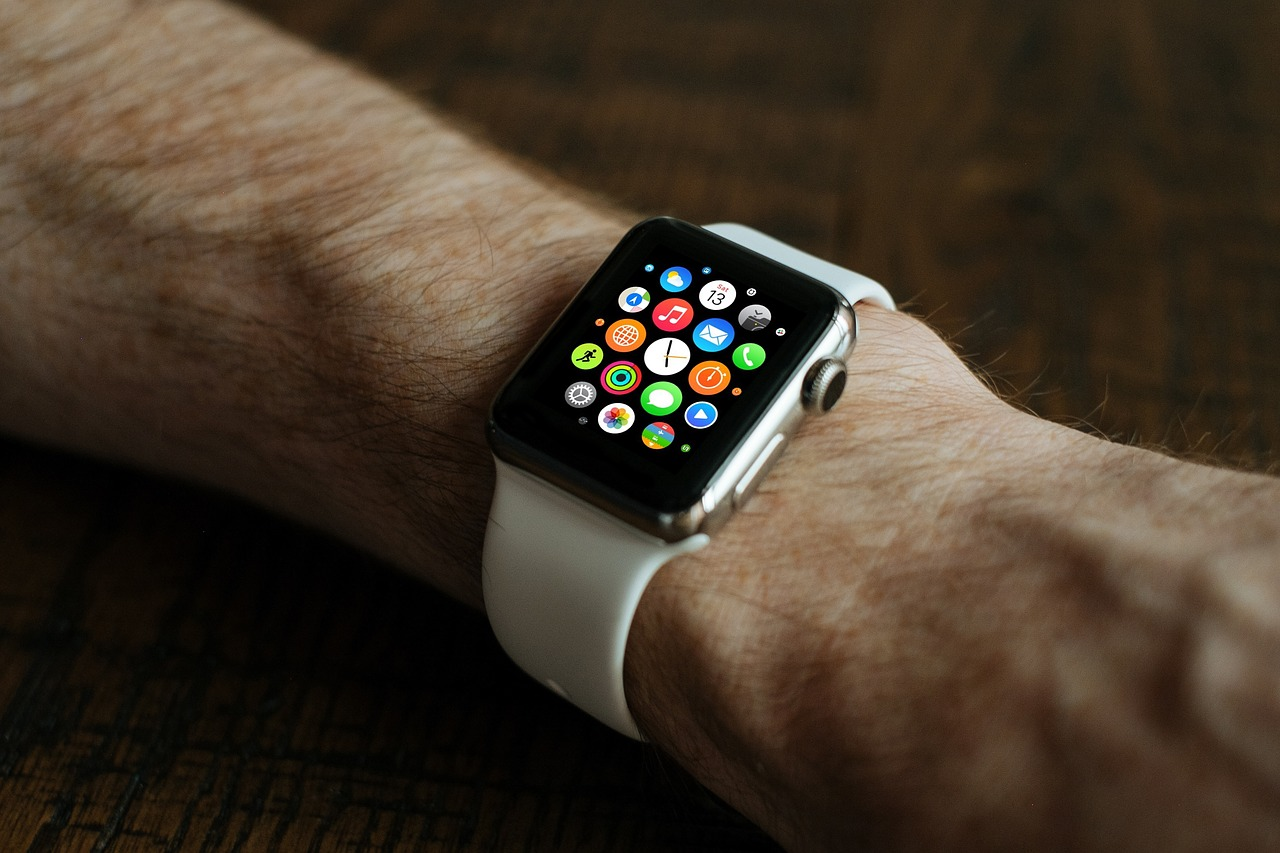
\includegraphics[width=\textwidth]{res/smart_watch}
        \caption{A smart watch}
        \label{fig:smart_watch}
    \end{subfigure}
    ~
    \begin{subfigure}[b]{0.3\textwidth}
        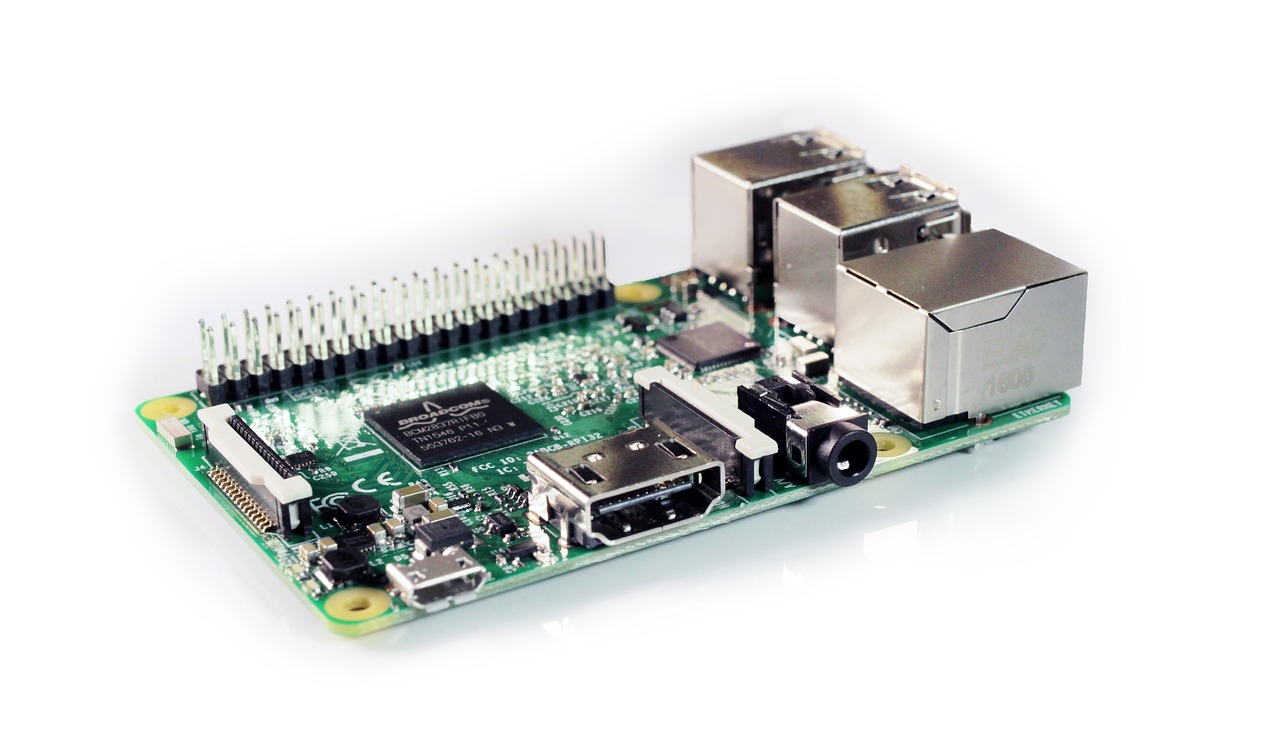
\includegraphics[width=\textwidth]{res/raspberry_pi}
        \caption{A raspberry pi}
        \label{fig:raspberry}
    \end{subfigure}
    \caption{Smart objects (Source: \url{pixabay.com})}\label{fig:smart_objects}
\end{figure}

While it seems pretty straightforward, there does not seem to be a fine line of what exactly smart objects refer to. They may refer to the actual small device with processing and interacting capacity, or the bigger entity that is a physical object made "smart" by the addition of a sensor or actuator. In our case we will consider the latter definition of what an IoT device is. Also in this thesis, we will often employ the terms motes, nodes, devices, smart objects or things to define the same concept. \\

\todo[inline]{Add numbers}
Those devices are quite limited also in term of resources. Those are small embedded devices with low power cpu and a limited memory size. Also they are not plugged meaning they rely mainly on their battery. To maximize the battery lifetime, they often switch between awake phases, where the mote is able to communicate and execute process, and sleep phases, where the mote does nothing. Additionally, their wireless range do not permit them to often communicate directly with all members of the network. This is why most of the IoT networks are organized in a hop-by-hop fashion. \\

(source : theinternetofthings.pdf, McKensey Quarterly)
The main purpose of smart objects is automation, to replace human intervention for specific computations and data collection. Obviously, they allow the \textit{collection} of bigger loads of data at a faster pace. Once data is collected, the next step is to make actual conclusions about data information. From that point, according to those computations, instructions are passed through the IoT network and the network can enter the process of modifying the physical world through actuators, in an automated fashion and again with no human intervention once the IoT network is set up.\\

To go along with automation, the Internet of Things aims at \textit{optimizing} how it affects the physical world, in terms of energy consumption efficiency, timing, accuracy, etc.

\section{Challenges of The IoT}

https://datafloq.com/read/three-major-challenges-internet-of-things/83 : cet article parle de trois gros challenges pour l'iot : shared standards and infrastructures, data control and access, data security.\\

\subsection{Lack of Standard Architecture}

The main challenges of the Internet of Things is to define a standard architecture. This is actually the main reason why it has not been fully deployed yet. Several characteristics are needed for the IoT to be deployed, and they should be included in the standard infrastructure. The characteristics needed are distributivity, interoperability (devices from different companies being able to communicate, with standardized protocols), scalability (huge amount of smart objects communicating), resources scarcity (power and consumption are limited on each device), and security. 


Main source : architecting the internet of things : state of the art.\\


"Its success relies greatly on a well-defined architecture that will provide scalable, dynamic, and secure basement to its deployment. In fact, several challenges stand between the conceptual idea of IoT, and the full deployement of its applications into our daily life. IoT deployment is closely related to the establishment of a standard architecture. This architecture should support future exten- sions, and covers IoT characteristics such as distributivity, interoperabil- ity, and scalability. A well defined, scalable, backward compatible, and secure architecture is required to bring the IoT concept closer to reality. In the literature, several architectures have been proposed. Nevertheless, each architecture brings a share of drawbacks, and fails covering all IoT characterisitcs. In this chapter, we review the main proposed architec- tures for the Internet of Things, highlighting their adequacy with respect to IoT requirements."\\

\subsection{The IoT, Not Totally Deployed Yet?}

Most existing applications using the Internet of Things have been developed privately. Companies, developers, researchers have developed some specific solutions using the Internet of Things. However, those solutions are more specific, and hence optimized, for one particular application.\\
\section{Network Organization}
\todo[inline]{Talk about the different organizations that an iot network can take.}

\subsection{Wireless Sensor Networks}

(en.wikipedia.org/wiki/Wireless\_sensor\_network),\\

The main kind of IoT network we have focused on are Wireless Sensor Networks. While our solution fits most types of IoT networks, we have decided to mainly focus on WSNs because they are the most constraining types(développer?).\\

(per Connecting iot objets with IP book)
The idea behind \textit{Wireless Sensor Networks} (\textit{WSN} in shortened form) is having small sensors collecting pertinent data from the physical world, communicating wirelessly to other sensors and in the end to a base station where all the data is collected and stored for further processing. Sensors not capable of directly transmitting information to the base station send their data to other sensors capable of relaying the information towards it (AJOUTER UNE IMAGE DE WSN?), in a hop by hop fashion.\\

Wireless Sensor Networks are regularly used for environmental conditions monitoring such as wild fire tracking, agriculture management, humidity and temperature monitoring in forests, effect of global warming on glacier structures, air pollution monitoring, and many more. They are also used in the industrial field such as in data centers, mainly to monitor the temperature of racks.  \\

(en.wikipedia.org/wiki/Sensor\_node),
The components of WSNs are "\textit{Wireless Nodes}" or "Motes". WSNs may be composed of a few hundreds to thousands of nodes, each node being conneted to one or several sensors. In addition to sensors, those nodes are also equipped with a microcontroller, a radio transceiver, memory, and a power source (a battery). The sensors are responsible for capturing data from the environment, especially when there is a change in an environmental condition such as temperature or humidity. (The continual analog signal produced by the sensors is digitized by an analog-to-digital converter and sent to controllers for further processing). Sensors are usually very small and thus consume a very low amount of battery power. The \textit{microcontroller} is responsible for peforming specific tasks and processing the data collected by the sensor, but also controlling other components of the node. The transceiver is used for communication purposes, mainly sending and receiving data using specific. It is often of the form of a radio or infrared. Transceivers have the particularity of both being able to send and receive data. Finally, the power source provides power supply instead of mains supply. The power source is thus in the form of a battery, it is consumed when the node is sending the environment, communicating with other sensor nodes, and doing some data processing. All of the components are designed to be as little power-consuming as possible. Having nodes not connected to mains power is an advantage because of not having to be plugged to a power supply (when the physical world makes it hard to have some, in moutains for example), but with such an advantage come resource constraints as we will explain later.  \\

The main challenges of WSNs are Data transmission, resource constraint, and security. First, nodes must send their data to the server. As discussed earlier, each node may not have the server in their sending range because of a lack of power, thus they must send their data to an intermediate node relaying the information. Moreover, limited battery, must stay idle, ENERGY HARVESTING etc. Puis security.\\

((((((Each such sensor network node has typically several parts: a radio transceiver with an internal antenna or connection to an external antenna, a microcontroller, an electronic circuit for interfacing with the sensors and an energy source, usually a battery or an embedded form of energy harvesting. A sensor node might vary in size from that of a shoebox down to the size of a grain of dust, although functioning "motes" of genuine microscopic dimensions have yet to be created. The cost of sensor nodes is similarly variable, ranging from a few to hundreds of dollars, depending on the complexity of the individual sensor nodes. Size and cost constraints on sensor nodes result in corresponding constraints on resources such as energy, memory, computational speed and communications bandwidth. The topology of the WSNs can vary from a simple star network to an advanced multi-hop wireless mesh network. The propagation technique between the hops of the network can be routing or flooding.)))))\\

(source : architecting the iot page 6) 
(((((
Sensor networks consist of a certain number, which can be very high, of sens- ing nodes communicating in a wireless multi-hop fashion (Figure 2). In general, nodes report their sensing results to a small number of special nodes called sinks (or base stations). A lot of effort has been undertaken by the scientific commu- nity on sensor networks. Indeed, many work have addressed several problems at the different layers of the protocol stack. In these works, the main issues concern energy efficiency (which is a limited resource in WSN), scalability (the number of nodes can rise significantly), reliability (the system might be involved in critical applications), and robustness (nodes might be subject to failure) [17].


\chapter{ContikiOS - Cooja - Softwares a portee de main}

We will now discuss Operating Systems in the Internet of Things. As discussed earlier, objects in IoT Networks have limited capabilities, i.e. processing capacity and storage, and limited battery. It is thus preferred to have an operating system that is not demanding and as light as possible. \\

Though not ideal, a light version of Linux could be used. However, one requirement of working with smart objects is having the ability to react to \textit{Real-Time events}. In a situation where a smart sensor is used in a car to make its airbags open when a car crash occurs, the software in the said sensor must react to the crash almost instantly. In this case, we need a maximum time reaction to an event, otherwise the purpose of the object (and thus the airbag) is not met. A few operating systems have been developed to answer to the requirements of IoT objects, they are light, have a minimal set of functionalities, plus they guarantee time-bounded reaction to events. (source : Mobile and embedded systems, prof Sadre)\\

\subsection{The Contiki Operating System}

Among existing operating systems, we have chosen to use one that is called \textit{ContikiOS}. It is an open source operating system and it was developed in 2003. Contiki is quite light in terms of memory, processing speed, and communication bandwidth. It is preemptive.\\

\todo{WHY WE HAVE CHOSEN CONTIKI?}

\begin{itemize}
\item protothreads
\item Reduced C
\end{itemize}
wikipedia : "Contiki provides three network mechanisms: the uIP TCP/IP stack,[5] which provides IPv4 networking, the uIPv6 stack,[6] which provides IPv6 networking, and the Rime stack, which is a set of custom lightweight networking protocols designed for low-power wireless networks. The IPv6 stack was contributed by Cisco and was, when released, the smallest IPv6 stack to receive the IPv6 Ready certification.[7] The IPv6 stack also contains the Routing Protocol for Low power and Lossy Networks (RPL) routing protocol for low-power lossy IPv6 networks and the 6LoWPAN header compression and adaptation layer for IEEE 802.15.4 links.

Rime is an alternative network stack, for use when the overhead of the IPv4 or IPv6 stacks is prohibitive. The Rime stack provides a set of communication primitives for low-power wireless systems. The default primitives are single-hop unicast, single-hop broadcast, multi-hop unicast, network flooding, and address-free data collection. The primitives can be used on their own or combined to form more complex protocols and mechanisms.[8]"

\section{Cooja Simulating Software}
An existing tool called \textit{Cooja} has been developed on Contiki. Cooja is a simulation software (partly an emulator too) for Internet of Things networks. It has many features, such as allowing to build networks with different types of components (Sky motes, Z1 motes). Those components are Contiki nodes, i.e. nodes working through ContikiOS. Cooja allows to upload code to virtual motes, the same way Contiki code may be uploaded on physical. Cooja can either emulate nodes (the hardware of each component is entirely emulated), or create "Cooja nodes" where Contiki code is uploaded on, compiled and then executed on a simulation host. (Cooja allows to use non-Contiki nodes as well. Pertinent?). Cooja presents itself as a very useful software for our thesis, as it allows us to simulate large networks, and is quite useful when it comes to testing, since the uploading and compilation time of Contiki codes on the nodes in the Network we are testing and analyzing is faster than on real hardware. It also avoids physical material restriction.

\chapter{Monitoring tools for traditional networks}

When speaking of monitoring for traditional networks, two techniques come to mind: \textit{Netflow} and \textit{sFlow}. The two approaches have the common goal to give network administrators informations about the traffic that passes through their networks. However, they differentiate in the way they do so. In our solution, we were mainly inspired by Netflow as it is more light than sFlow in term of memory used.

\section{Netflow - A Traffic Collector}
\textit{Netflow} is a feature that was created by Cisco Systems and introduced on Cisco Routers. Netflow allows the collection of the IP traffic in networks, and thus monitoring network traffic. Information such as Source and Destination addresses (defined as "Flows) and Traffic volume can be retrieved and further analyzed.\\

There are three components when having Netflow set up : the Flow Exporter, the Flow Collector(s), and the analysis application (reference wikipedia/article). The Flow Exporter collects packets and forms what we call flows (having various definitions according to the version of Netflow used). Flows represent a stream of packets sharing common attributes (such as source and destination addresses). The exporter records the flows into Netlow records and sends passes them onto the Flow Collector. After reception, the Flow Collector will store the flow records received from the Exporter. The data stored can then be analyzed by applications, hence having statistics of traffic exchanges in a particular network. The Fig.\ref{fig:netflow} illustrate the different parties in a Netflow process.\\

\begin{figure}
  \centering
  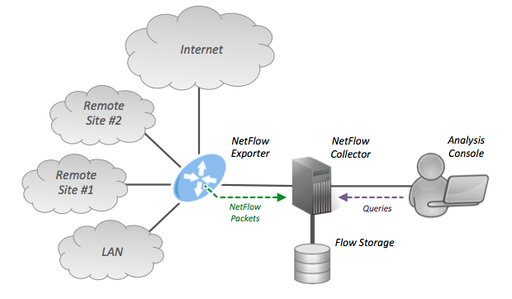
\includegraphics[width=\textwidth]{res/netflow.png}
  \caption{Netflow}
  \label{fig:netflow}
\end{figure}

The version of Netflow that we are quite interested in, is the Netflow version 10 or \textit{IPFIX} \cite{claise2013rfc}. This version is an IETF (Internet Engineering Task Force) protocol whereas the previous versions are proprietaty protocols of Cisco. IPFIX is template based meaning that contrary to previous versions of Netflow (excluded version 9 which is also template based), the netflow records can vary to suit the need of the administrators or organizations. The template permit to define what we want to retrieve and by the same occasion define what we consider to be a flow. An organization could consider a flow to be 3-uple: source ipv6 address, destination ipv6 address, number of octets exchanged. While another one could consider a flow to be the 4-uple: source ipv6 address, destination ipv6 address, number of octets exchanged, number of packets exchanged. \\

The IANA (Internet Assigned Numbers Authority)

\todo[inline]{Ajouter des détails techniques ici sur Netflow}.\\

Having defined what Netflow is, the main goal here is to be able to use Netflow on an IoT device. In the Introduction section, we explained that our main goal was to analyze the traffic of an IoT Network and retrieve pertinent information such as the volume exchanged in the network, and its topology. Netflow is basically what we want to achieve in terms of data collecting. However, it has not been implemented by Cisco for IoT devices. Our task is to implement Netflow for an IoT device, using predefined data formats that will allow us to collect the information we are interested in (battery level, source and destination addresses, packet volume, etc.). In the Solution section (fourth section?), we will describe in more details how we used Netflow in IoT Networks as a solution to our monitoring task.

\section{sFlow}

\chapter{Current Monitoring Tools for IoT}
